
\section{HML without recursion}

\begin{verbatim}
Process s: RecX(a?.b?.RecY((b?.Y + a?.X)))
Process t: RecX(a?.RecY((b?.Y + b?.a?.X)))
Process v: RecX(a?.(b?.b?.RecY((b?.Y + a?.X)) + b?.RecY((b?.Y + a?.X))))

s isn't  bisimilar to t due to formula f= [a][b]<a>tt
s satisfy f: true
t satisfy f: false


s isn't  bisimilar to v due to formula f= [a]<b>[a]ff
s satisfy f: false
v satisfy f: true


t isn't  bisimilar to v due to formula f= [a]<b>[b]ff
t satisfy f: true
v satisfy f: false
\end{verbatim}

\begin{figure}[htb]
  \centering
  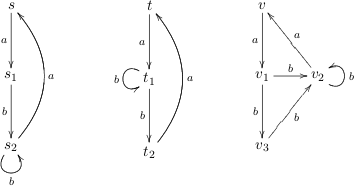
\includegraphics{qualitative-project/not-bisimilar-processes.png}
  \caption{Three not bisimilar processes}
  \label{fig:not-bisimilar-processes}
\end{figure}
